% --- [ Interval Method ] ------------------------------------------------------

\subsection{Interval Method}
\label{sec:interval_method}

The Interval method is a control flow recovery method that relies on graph \textit{intervals} to locate loops in control flow graphs. To distinguish the nesting level of loops, the notion of a \textit{derived sequence of graphs} is used; as further explained below.

% ~~~ [ Interval ] ~~~~~~~~~~~~~~~~~~~~~~~~~~~~~~~~~~~~~~~~~~~~~~~~~~~~~~~~~~~~~

An \textbf{Interval} $I(h)$ with header node $h$ is a maximal single-entry subgraph in which $h$ is the only entry node and all cycles contain $h$. Importantly, a control flow graph $G$ can always be partitioned into a unique set of intervals \cite{structuring_algorithm_for_decompilation}. To give a concrete example, the control flow graph presented in figure \ref{fig:interval} has been partitioned into its unique set of intervals \textbf{I(B1)}, \textbf{I(B6)} and \textbf{I(B13)}.

\begin{figure}[htbp]
	\centering
	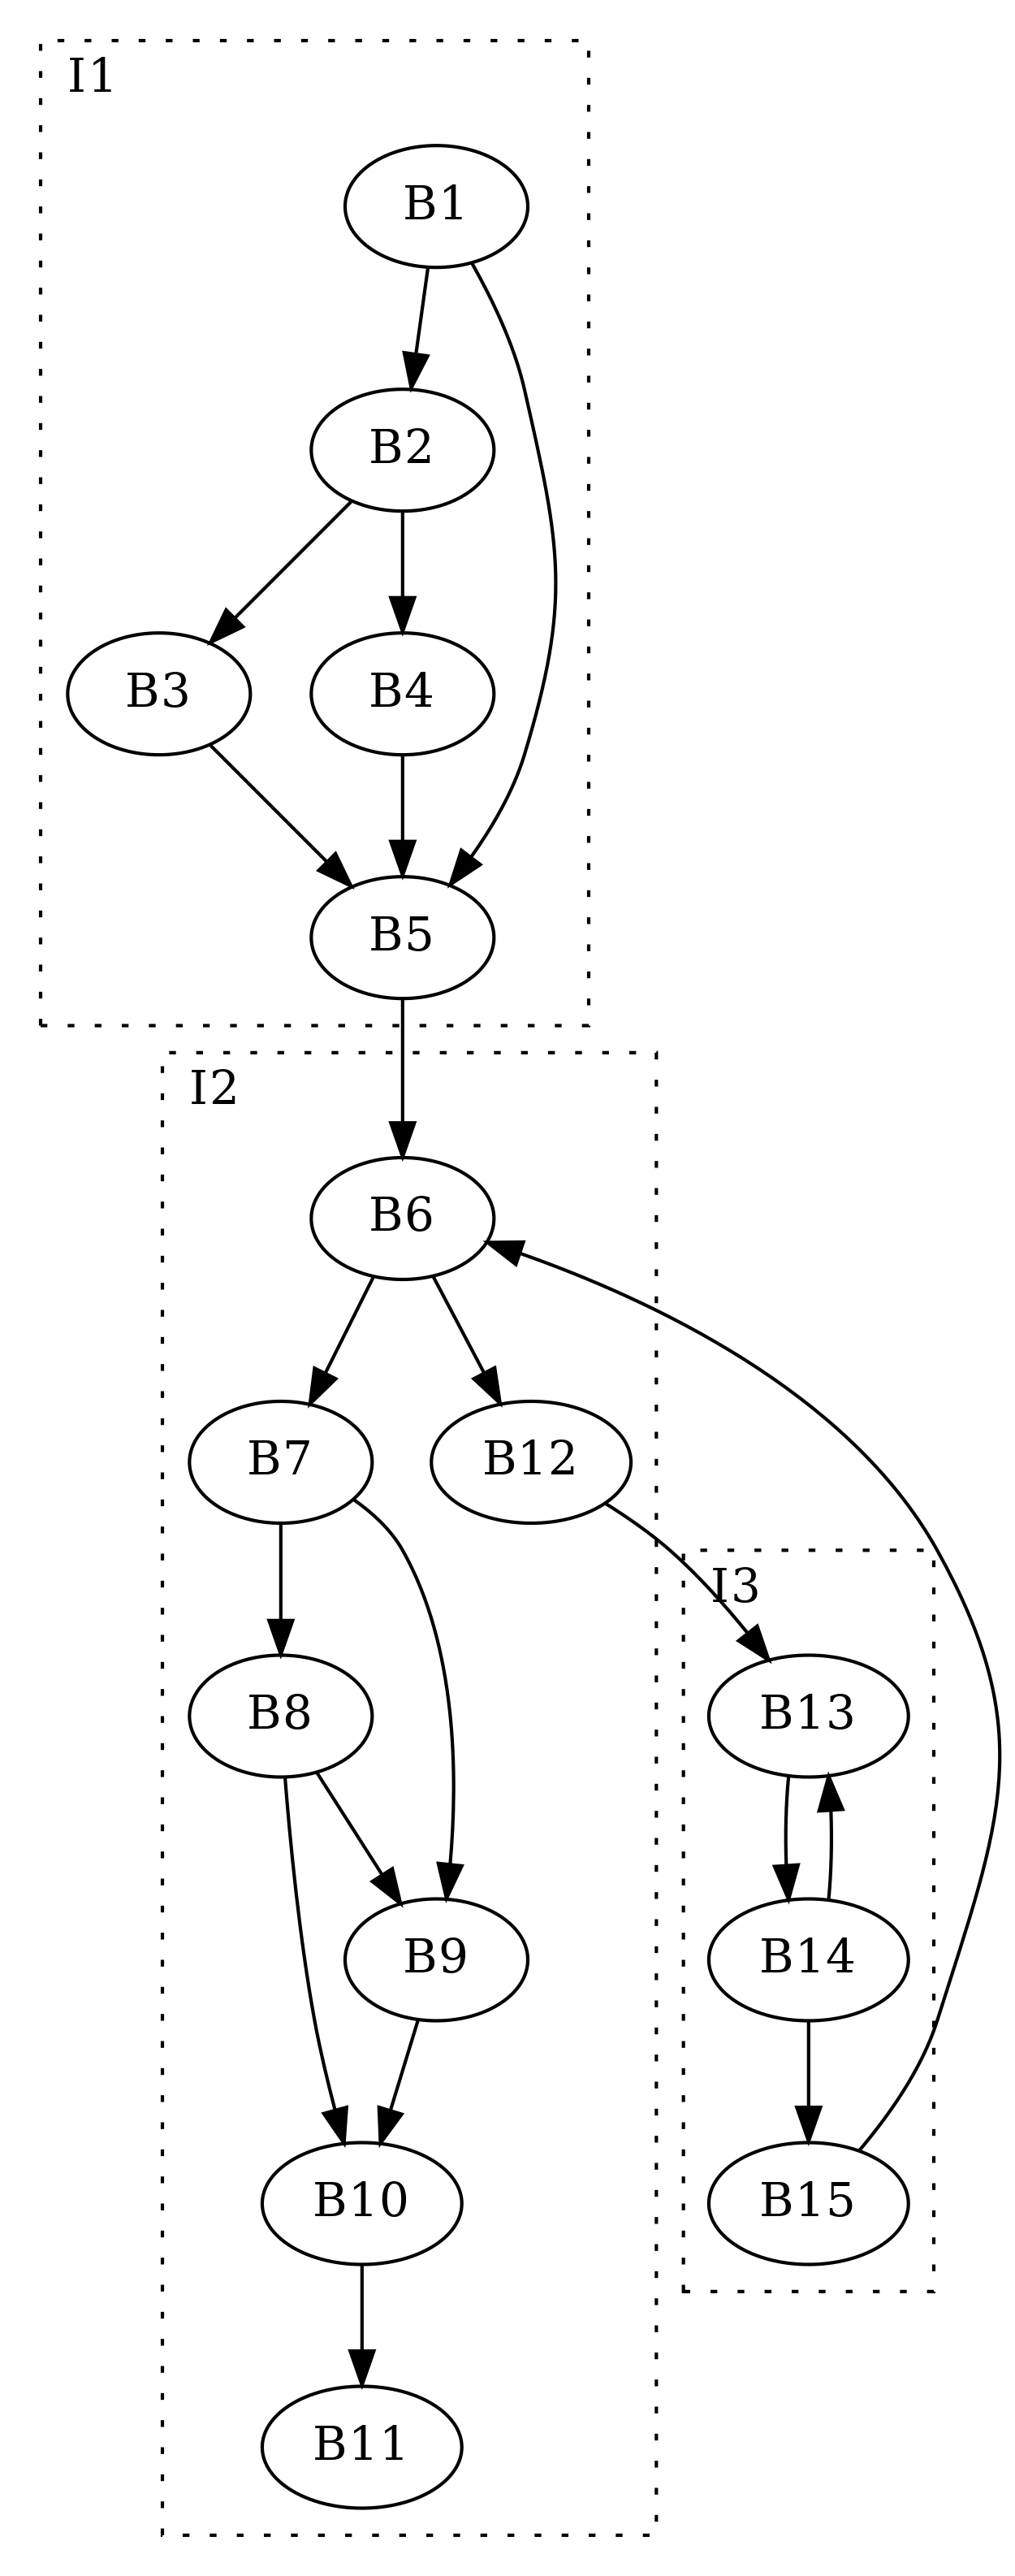
\includegraphics[width=0.3\textwidth]{inc/appendices/vocabulary/interval.png}
	\caption{The unique set of intervals \textbf{I(B1)}, \textbf{I(B6)} and \textbf{I(B13)} (also referred to here as \textbf{I1}, \textbf{I2} and \textbf{I3}, respectively) outlined in a control flow graph; adapted from figure 2 of C. Cifuentes' \textit{Structuring Decompiled Graphs} \cite{structuring_decompiled_graphs}.}
	\label{fig:interval}
\end{figure}

% ~~~ [ Derived Sequence of Graphs G^1...G^n ] ~~~~~~~~~~~~~~~~~~~~~~~~~~~~~~~~~

Given a control flow graph $G$ a \textbf{derived sequence of graphs}, $G^1 \dots G^n$, may be obtained by a recursive process of collapsing intervals. The first order graph $G^1 = G$. The second order graph $G^2$ is obtained by collapsing each interval in $G^1$ into a dedicated node (in other words, each node of $G^2$ denotes an interval of $G^1$). The node of a collapsed interval $I(h)$ has incoming edges from the immediate predecessors of the header node $h$ not part of the interval, and outgoing edges to the immediate successors of the exit nodes of $I(h)$ not part of the interval. The intervals of $G^2$ are collapsed and the process is repeated until $G^n$ is a single node or an irreducible graph; as illustrated in figure \ref{fig:derived_sequence_of_graphs}.

\begin{figure}[htbp]
	\centering
	\begin{subfigure}[b]{0.30\textwidth}
		\centering
		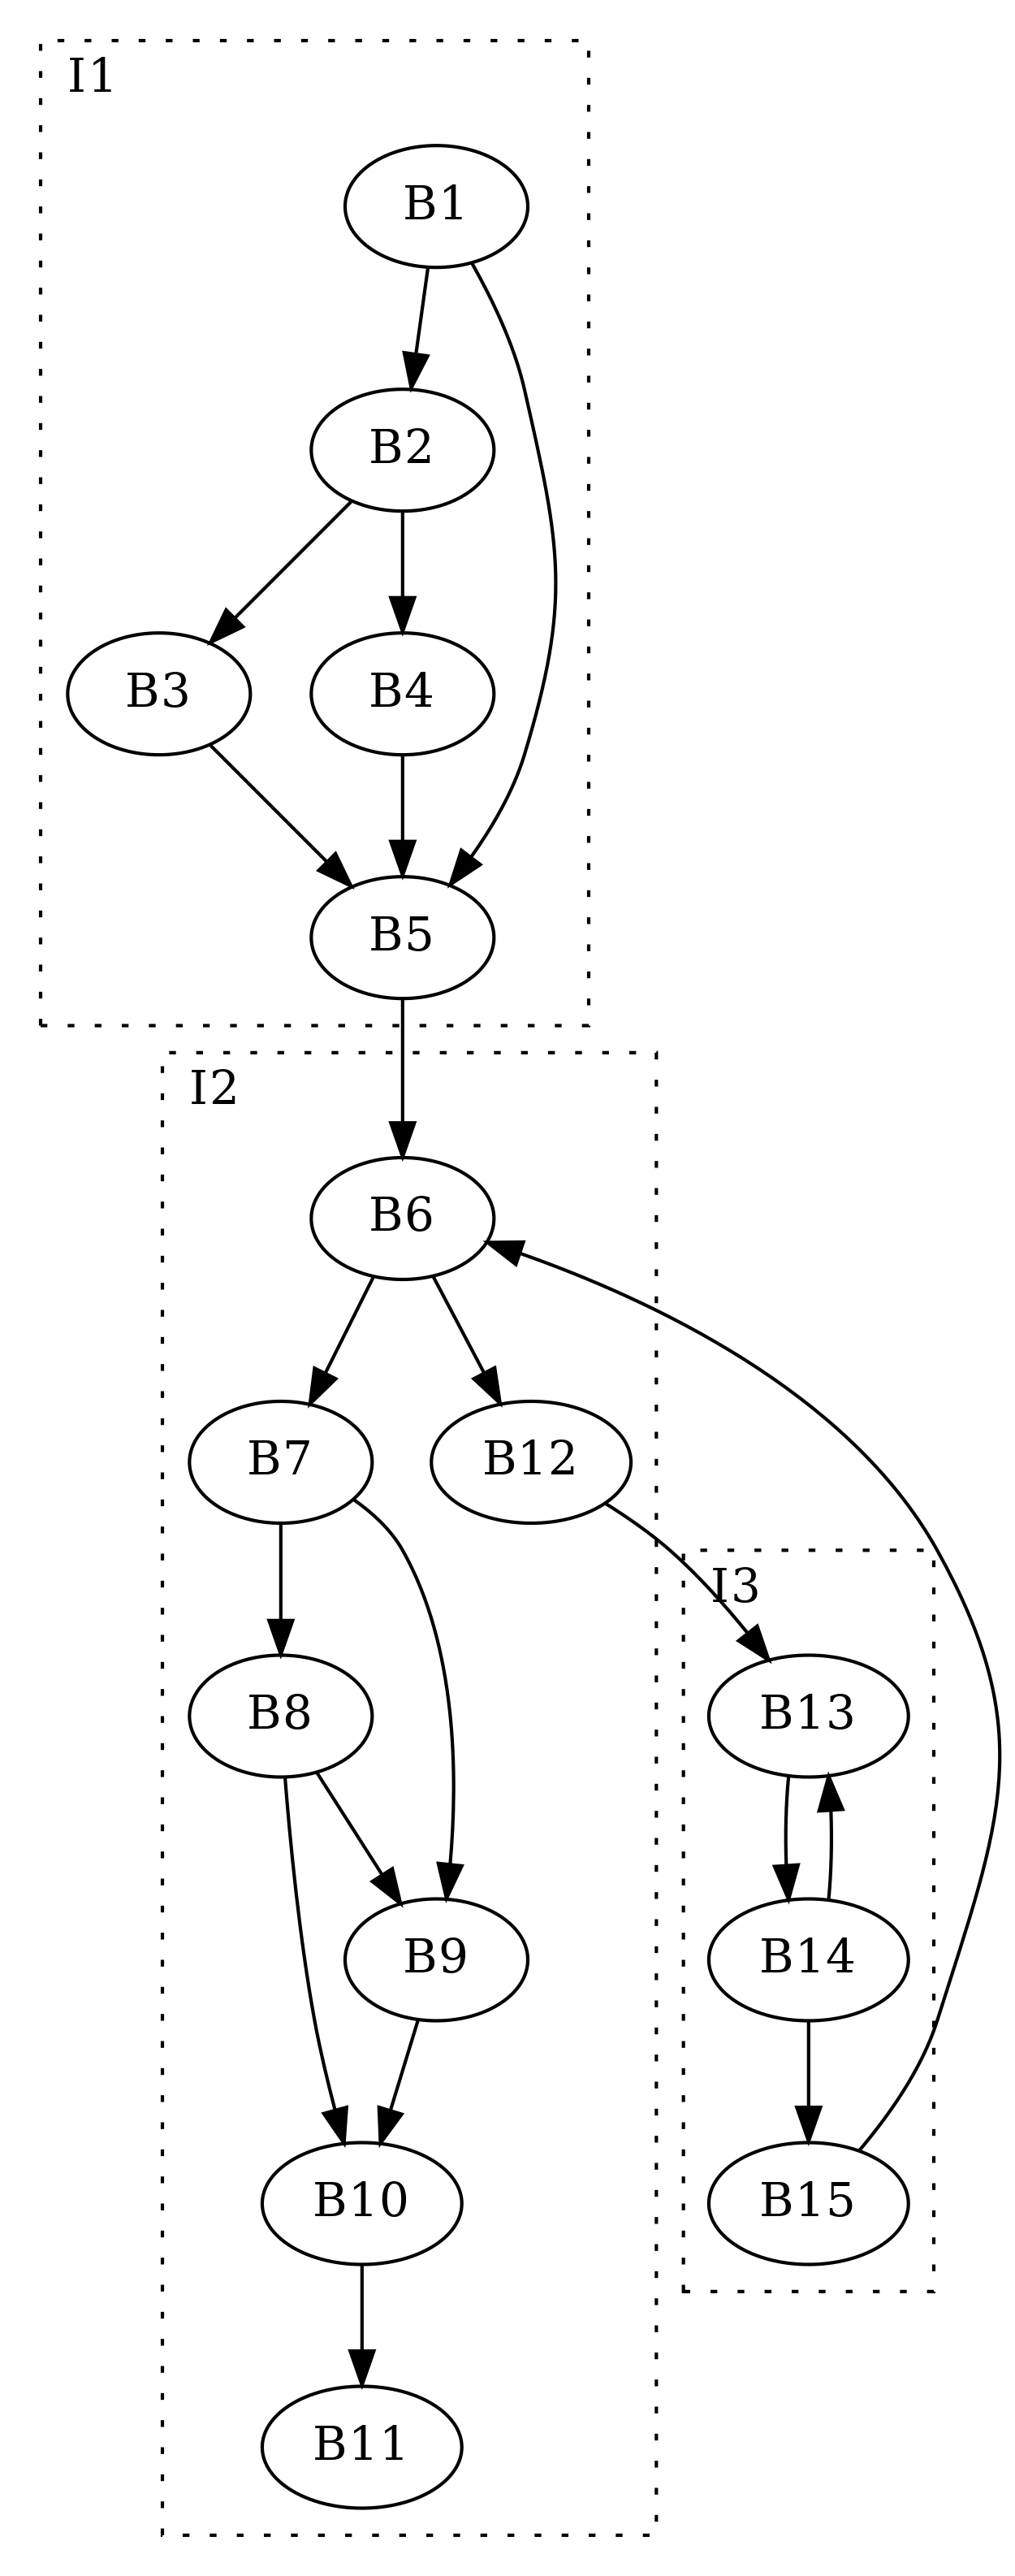
\includegraphics[width=\textwidth]{inc/3_background/interval_method/derived_sequence_of_graphs/G_1.png}
		\caption{$G^1$}
	\end{subfigure}
	\qquad
	\begin{subfigure}[b]{0.12\textwidth}
		\centering
		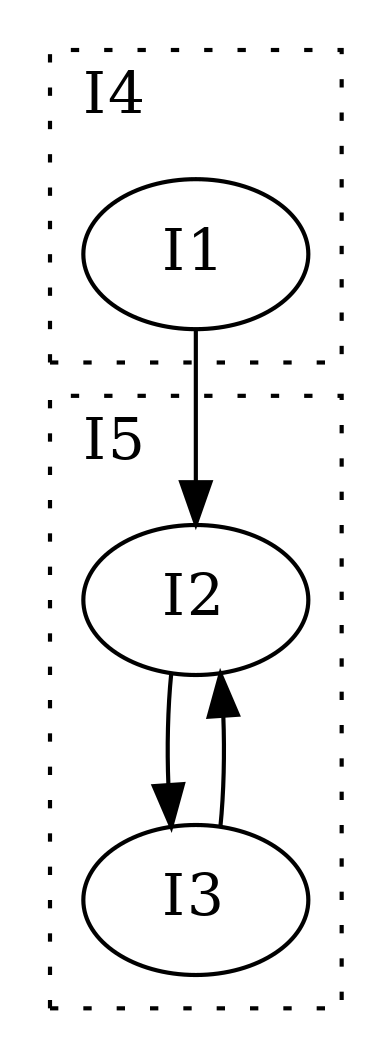
\includegraphics[width=\textwidth]{inc/3_background/interval_method/derived_sequence_of_graphs/G_2.png}
		\caption{$G^2$}
	\end{subfigure}
	\qquad
	\begin{subfigure}[b]{0.12\textwidth}
		\centering
		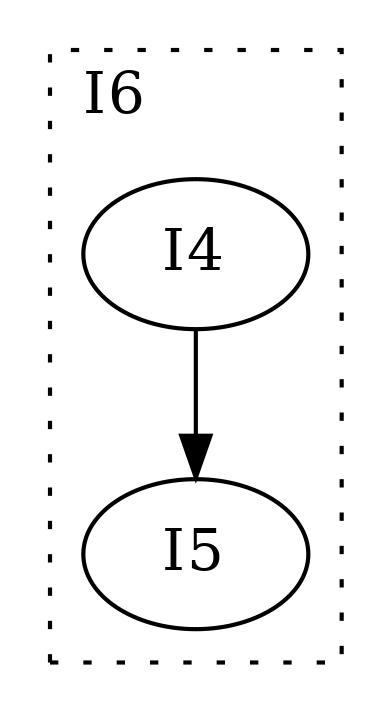
\includegraphics[width=\textwidth]{inc/3_background/interval_method/derived_sequence_of_graphs/G_3.png}
		\caption{$G^3$}
	\end{subfigure}
	\qquad
	\begin{subfigure}[b]{0.08\textwidth}
		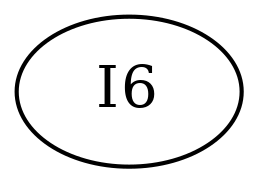
\includegraphics[width=\textwidth]{inc/3_background/interval_method/derived_sequence_of_graphs/G_4.png}
		\vspace{2em}
		\caption{$G^4$}
	\end{subfigure}
	\caption{Derived sequence of graphs, $G^1, ..., G^n$; adapted from figure 3 of C. Cifuentes' \textit{Structuring Decompiled Graphs} \cite{structuring_decompiled_graphs}.}
	\label{fig:derived_sequence_of_graphs}
\end{figure}

% ___ [ Structuring of Loops ] _________________________________________________

\subsubsection{Structuring of Loops}

The unique property with intervals .... \todo{TODO: continue}.

\begin{table}[htbp]
	\begin{center}
		\begin{tabular}{|l|l|l|l|}
			\hline
			\textbf{Header node} & \textbf{Latch node} & \textbf{Loop type} \\
			\hline
			unconditional & unconditional & endless loop                         \\
			\hline
			conditional   & unconditional & pre-test loop                        \\
			\hline
			unconditional & conditional   & post-test loop                       \\
			\hline
			conditional   & conditional   & pre-test loop with conditional break \\
			\hline
		\end{tabular}
	\end{center}
	\label{tbl:loop_classification}
	\caption{Classification of loop type based on the header and latch node of the loop.}
\end{table}

% ___ [ Structuring of 2-way Conditionals ] ____________________________________
% ___ [ Structuring of N-way Conditionals ] ____________________________________
% ___ [ Structuring of Compound Conditionals ] _________________________________

For a complete example using the Interval method to recover the high-level primitives
of a C source program by analyzing the control flow graph produced from the LLVM IR
representation of a source program, refer to appendix \ref{app:interval_example1}.
